\documentclass{article}
\usepackage[spanish,es-lcroman,activeacute] {babel}
\usepackage[utf8]{inputenc}
\usepackage{hyperref}
\usepackage{graphicx}
\usepackage[margin=2cm]{geometry}
\usepackage{subcaption}
\usepackage{caption}
\usepackage{amsmath}
\usepackage{color}
\usepackage{float}
\usepackage{parskip}

%Eliminar bordes rojos de los hipervinculos
\hypersetup{pdfborder=0 0 0}

\setlength{\parskip}{3.1mm plus2mm minus2mm}

\title{Resumen Artículo científico: Generación de $\beta$-esqueletos con cómputo paralelo \cite{beta}}
\author{Camilo Andrés Rivera}
\date{12 de Junio de 2015}

\begin{document}
\maketitle

Los $\beta$-esqueletos son grafos, en la mayoría de casos 2-D, en el cual dos puntos estarán conectados dependiendo de su ubicación relativa (satisfaciendo ciertas condiciones geométricas) y del parámetro $\beta$. Este tipo de algoritmos es usado en una gran variedad de aplicaciones, entre ellas el aprendizaje de máquinas para problemas de clasificación geométrico, y para la generación de mallas de triangulación, por ejemplo para simulaciones de elementos finitos. Este método también es usado ampliamente en el tratamiento de imágenes para la reconstrucción de formas a partir de puntos sobre la frontera, por ejemplo reconstrucción de rostros.

Dado que la cantidad de puntos puede aumentar de gran manera dependiendo de la aplicación, es importante la generación de algoritmos óptimos para la obtención del grafo. Este es el caso de \cite{unoados} en donde se muestra un algoritmo óptimo para la construcción del \textit{Relative Neighborhood Graph} para el caso $1\leq\beta\leq2$ con un tiempo de $\mathcal{O}(n)$, usando una triangulación Delaunay, en la cual ningún punto puede estar dentro de la circunferencia circunscrita por cada triángulo, como se muestra en la Figura \ref{fig:delaunay}. Por otro lado, en \cite{menosdeuno}, se muestra un algoritmo $\mathcal{O}(n^2)$ para el caso de $\beta<1$.

\begin{figure}[H]
\centering
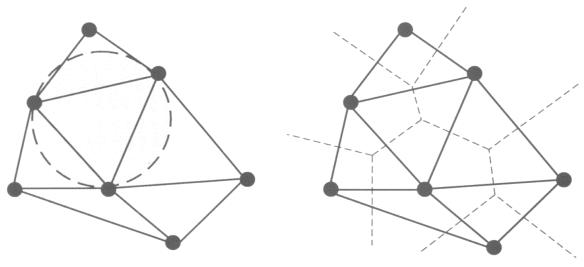
\includegraphics[width=0.6\textwidth]{imagen}
\caption{Triangulación de Delaunay con su estructura de Volonoi}
\label{fig:delaunay}
\end{figure}

Para el caso del artículo elegido \cite{beta}, se tiene que los procesadores usados para la programación en paralelo seguían un modelo CREW\_PRAM, el cual quiere decir que múltiples procesadores podían leer una célda de memoria simultáneamente pero sólo uno podía escribirla (\textit{Concurrent read exclusive write}: CREW). El término PRAM viene de Parallel RAM o \textit{parallel random access memory}. Se nombran dos usos de los algoritmos paralelos, de las cuales la primera trata de encontrar un $\beta$-\textit{spectrum}, que se le llama al conjunto de todos los vértices que pertenecen al $\beta$-esqueleto. El pseudo-algoritmo diseñado para la generación del $\beta$-\textit{spectrum} fue: construir la triangulación de Delaunay, construir el conjunto de árboles de eliminación (bosque de eliminación), extraer los polígonos conectados a cada árbol de eliminación, extracción de polígonos centrales y finalmente la estructura de Voronoi. Esta última, como se ve en la parte derecha de la Figura \ref{fig:delaunay}, se refiere a las fronteras a partir de las cuales se está más cerca de un punto en particular en vez de otro.

Para el caso del uso de paralelismo para la generación de esqueletos, se asignan los vértices de los árboles de eliminación a procesadores, alternando una clasificación entre procesadores ``blancos'' y ``negros'', los cuales están determinados de cierta manera en la que un procesador blanco puede tener dos predecesores negros pero sólo un sucesor negro. La idea es que en cada iteración para cada árbol de eliminación, se revisa algún vértice correspondiente a un procesador blanco elimina todos los bordes del siguiente grupo de negros, en dado caso se elimina el grupo de procesadores negro y se juntan los blancos con los siguientes. El proceso se realiza similarmente con los conjuntos de procesadores negros. Al eliminar un grupo, se realiza la conexión de los grupos adyacentes (ya sean blancos o negros). Para el caso a $\beta\in[1,2]$ se demuestra que este algoritmo tiene una velocidad de convergencia de $\mathcal{O}(\log^2n)$.


%\nocite{*}
\bibliographystyle{apalike} %ORDENADOS!
\bibliography{science}
\end{document}	